% Drawing 93/09-1 -- folder 93, batch 09, archive page 168 (PDF page 169).
% Transcription: entre les deux lignes de bases, des flèches obliques relient $x^{k}$ à $x^{k-1}dx$ (la différentielle, avec un coefficient noté sous la troisième flèche) ; $x^{p-1}dx$ est seul à ne pas être atteint, et la flèche partant de $1$ aboutit à un point (zéro).
% Kind: differential arrows between the bases of Omega^0 and Omega^1. Method 2 (schematic redraw from the facsimile). Status: ok.
% Notes: The two lines of bases (1, x, x^2, ..., x^{p-2}, x^{p-1} above; dx, x dx, x^2 dx, ..., x^{p-1}dx below) with oblique arrows from x^k down to x^{k-1}dx; the arrow from 1 ends at a point (zero); the coefficient "2" under the third arrow; the last arrow (heavy) comes from x^{p-1}. The basis labels are placed as on the page.
% Coordinates: 1 unit = 1 mm = 1/100 of the crop width (bbox in page fractions: [0.5, 0.42, 0.95, 0.5]).
% Redrawn by Claude (claude-opus-5-5), issue #73, 2026-11-07; not checked by a human; not compiled (no TeX in the session).
% Rights: reproduces part of the work -- behind RENDER_TRANSCRIPTS, never published by itself.
\documentclass[tikz,border=3pt]{standalone}
\usepackage{amsmath,amssymb}
\usetikzlibrary{patterns,arrows.meta}
\tikzset{pencil/.style={black!45}, struck/.style={black!35}, mark/.style={circle,draw,inner sep=1.3pt}, pt/.style={circle,fill,inner sep=0.9pt}, opt/.style={circle,draw,fill=white,inner sep=1.1pt}}
\begin{document}
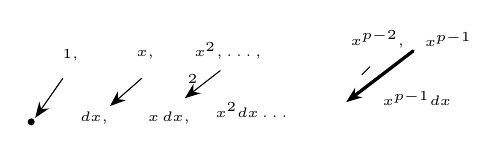
\begin{tikzpicture}[x=1mm,y=1mm,line cap=round,line join=round,font=\scriptsize]
\node[inner sep=1pt] at (31,-10) {\tiny $1,$};
\node[inner sep=1pt] at (40.5,-10) {\tiny $x,$};
\node[inner sep=1pt] at (51,-9.5) {\tiny $x^2,\ldots,$};
\node[inner sep=1pt] at (70,-8) {\tiny $x^{p-2},$};
\node[inner sep=1pt] at (79,-8) {\tiny $x^{p-1}$};
\node[inner sep=1pt] at (34,-18) {\tiny $dx,$};
\node[inner sep=1pt] at (43.5,-18) {\tiny $x\,dx,$};
\node[inner sep=1pt] at (54,-17) {\tiny $x^2dx\ldots$};
\node[inner sep=1pt] at (75,-15.5) {\tiny $x^{p-1}dx$};
\draw[-{Stealth[length=2mm]}] (30,-13) -- (26.5,-18);
\node[pt] at (26,-18.5) {};
\draw[-{Stealth[length=2mm]}] (40,-13) -- (36,-16.5);
\draw[-{Stealth[length=2mm]}] (50,-12) -- (45.5,-15.5);
\node[inner sep=1pt] at (46.5,-13) {\tiny $2$};
\draw[-{Stealth[length=2mm]},very thick] (74.5,-9.5) -- (66,-16);
\draw (69,-11.5) -- (68,-12.5);
\end{tikzpicture}
\end{document}
